\chapter{Aplicações do net.map}
\label{chp:applications}

Este capítulo tem por objetivo mostrar duas implementações reais do sistema apresentado neste documento, mostrando que o sistema não existe apenas no campo teórico e afirmando seu potencial impacto social e comercial.

\section{APScanner}

\textbf{APScanner} é um aplicativo Android feito para a aquisição e treinamento dos dados para o net.map. Nele é possível criar instalações e zonas, além de capturar os sinais de \textit{access points Wi-Fi} ao redor e enviá-los para o servidor do sistema. Também é capaz de mostrar a zona na qual o usuário se encontra no momento.
\\
As telas do aplicativo APScanner estão disponíveis no anexo \ref{anexo:telasApscanner}.

\section{EletricaGO}

Em julho de 2016 foi lançado ao redor do mundo o jogo de realidade aumentada Pokémon GO. Se trata de um jogo eletrônico \textit{free-to-play} voltado para \textit{smartphones}, onde os usuários andam pelas ruas buscando \textit{pokémons}, as criaturas existentes no jogo, utilizando para isso o GPS de seus \textit{smartphones}. Com mais de 500 milhões de downloads até novembro de 2016, o jogo se provou um sucesso comercial, e abriu as portas para que mais aplicações de realidade aumentada sejam desenvolvidas \cite{dapokemon}.
\par
Tendo em vista a popularidade do Pokémon GO, decidiu-se replicá-lo parcialmente para ser apresentado em conjunto com o resto deste projeto, mudando o contexto da aplicação. Chamado de \textbf{EletricaGO}, ao invés de funcionar em ruas e parques, funcionará dentro do prédio e Engenharia Elétrica da Escola Politécnica da USP. E ao invés de utilizar o GPS, utilizará o net.map, sistema apresentado neste documento.
\par
No EletricaGO, o usuário terá uma lista de algumas salas e ambientes do prédio de Engenharia Elétrica, e ao lado do nome de cada zona, um nome de um \textit{pokémon} que pode ser encontrado nessa zona. Ao chegar na zona, o usuário pode iniciar a captura \textit{pokémon}, conforme mostra a figura \ref{fig:telaEletericaGo}.

\begin{figure}[H]
  \centering
  \begin{minipage}[b]{0.7\textwidth}
    
    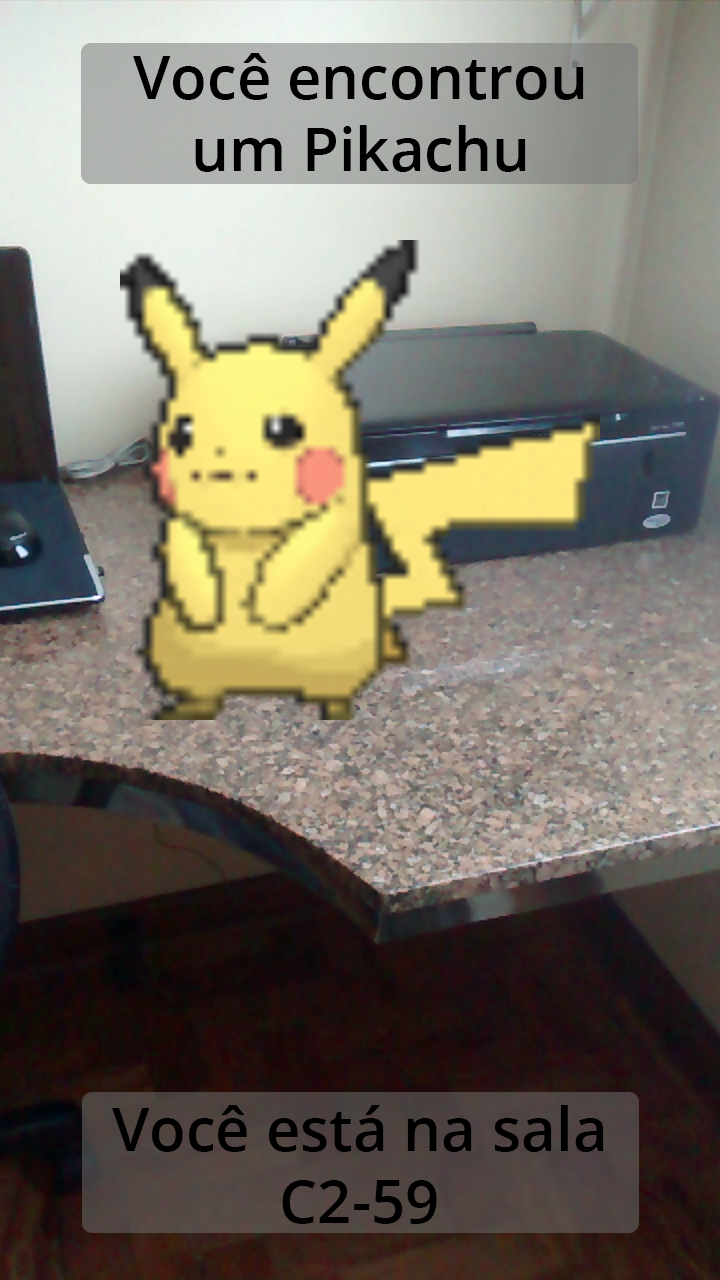
\includegraphics[width=\textwidth]{imagens/screenshots/eletricaGo.png}
    \caption{Tela do EletricaGO mostrando um \textit{Pokémon} na sala C2-59 do prédio de Engenharia Elétrica da POLI-USP}
    \label{fig:telaEletericaGo}
  \end{minipage}
\end{figure}